\def\theTopic{Descriptive Stats }
\def\dayNum{2}

\begin{center}
{\bf {\large Got Data?}}
\end{center}
 

Statistics is all about making sense of data, so we first need to pay
some attention to the main types of data we will be using.

\begin{enumerate}
  \item Which  variable is of a  different type?
    \begin{alist}
      \item  The cell phone carrier you use.
      \item  The monthly fee charged by your cell phone provider.
      \item  Whether your cell phone has buttons or touch screen.
      \item  The manufacturer of your cell phone.
    \end{alist}
     Circle the odd ball and explain why its different.
\begin{students}
    \vspace{1cm}    
\end{students}

\begin{key}
  {\it B.  It's numeric, not categorical.}       
\end{key}

\item Got it?  -- Let's just check again for the different data type.
  \begin{alist} \setcounter{alistctr}{4}
    \item Amount you spend on textbooks this term.
    \item Number of credits you're signed up for.
    \item How much student loan you'll take out this term.
    \item The area code of your phone number.
  \end{alist} Again circle one and explain.
\begin{students}
    \vspace{1cm}
\end{students}

\begin{key}
  {\it D.  Area code is categorical. Finding an average for the class
    makes sense for the others, but average area code is meaningless.}       
\end{key}
\item \label{summry}One thing we need to be comfortable with is
  summarizing data.  For each of the above variables, A through H, how
  would you summarize data collected from each person in class today?
\end{enumerate}
 \newpage

You've read about two main types of data:
\begin{list}{}{}
\item [\bf Quantitative] takes numeric values which we can average.
\item [\bf Categorical] falls into one of two or more categories.  The
  categories can have numeric labels (like zip codes), but it makes no
  sense to average them. (some call this ``Qualitative'', but we don't
  like to use two words starting with Q) 
\end{list}

\begin{enumerate} 
\setcounter{enumi}{3}
\item  For which variables on the previous page, A through H, would the
  {\bf mean} be informative?
\begin{students}
    \vspace{\fill}    
\end{students}

\begin{key}
  {\it B, E, F, G }
\end{key}
\end{enumerate}

   We also need to summarize categorical data, so we use proportions:
   the number in a certain category divided by the total number.

\begin{enumerate} 
\setcounter{enumi}{4}
\item  For which variables on the previous page, A through H would the
  {\bf proportions} be informative?
\begin{students}
    \vspace*{\fill}    
\end{students}

\begin{key}
  {\it A, C, D, H }
\end{key}
     
\end{enumerate}
  %\newpage
\begin{center}
  {\bf     Comparing Distributions} \vspace{-.2in}
\end{center}

 Now we'll focus on quantitative data.    \vspace{-.3in}
 \begin{enumerate}
\setcounter{enumi}{5}
 \item \label{center}
   Suppose you are choosing which professors' class to enroll
     in.  You have three choices, and have data on the grade
     distribution for each shown as histograms.  
     Which class seems to have the best grade distribution? Explain. \\
  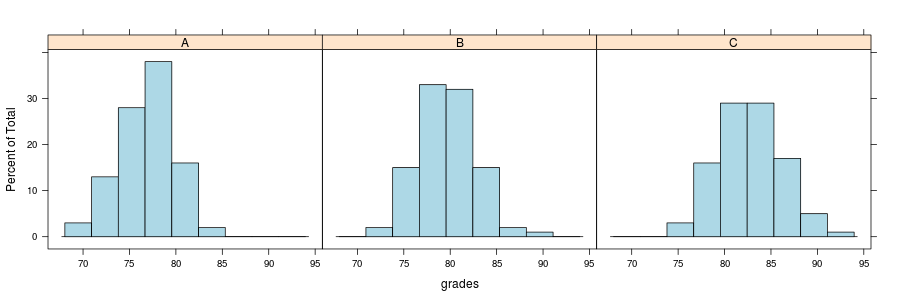
\includegraphics[width = .7\linewidth]{../../plots/3classGradeCompareMn.png}
\begin{students}
    \vspace{2cm}    
\end{students}

\begin{key}
  {\it Class C has the largest mean and median, so most will vote for it. }
\end{key}

\item  \label{skew} Here's another set of three distributions of exams scores.
     The density plots shown are essentially smoothed off histograms.
     Which do you prefer?  Explain why. 

   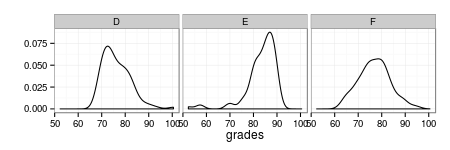
\includegraphics[width=.7\linewidth]{../../plots/3classGradeCompareSkw.png}
\begin{students}
    \vspace{2cm}    
\end{students}

\begin{key}
  {\it Class H has more A's than C's, so it's the wise choice.  I
    seems evenly split to high and low grades, while G seems to have
    lots of low grades.}
\end{key}

    
   \item  \label{spread}And here's a third set as a dot plot. Each point is one
     student's exam score -- stacked up when several people have the
     same score.   Which class do you prefer?  Explain the
     differences.  
     
    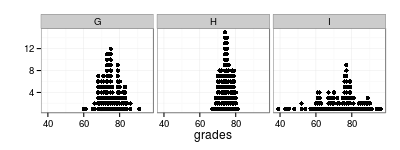
\includegraphics[width=.7\linewidth]{../../plots/3classGradeCompareSD.png}
\begin{students}
    \vspace{2cm}    
\end{students}

\begin{key}
  {\it The big difference here is in spread.  If you're an ``average''
  student, then you would like E because almost everyone gets a C and
  there's little chance of flunking.  If you are a good student, then
  F is more attractive since more people get A's in this class.}
\end{key}


  \item  When comparing distributions there are several things to consider:
    \begin{enumerate}
    \item  Comparing location or center (measured by mean or median)
      tells us which class did best ``on average''. 
    \item  Comparing spread (interquartile range or standard
      deviation) tells us which class is generally closest to its mean.
    \item  Comparing skew (could be left or right) to symmetric tells
      us which tail stretches out more.
      (Let's hope that there are more high grades than low ones.) 
    \end{enumerate}
    In the three problems above, which comparison were you making?
    For each set of comparisons, fill in center, spread, or skew. \\
    (\ref{center} )
\begin{students}
\underline{\hspace*{3cm}}\hfill 
\end{students}
\begin{key}
  \underline{\hspace*{1cm}}  {\it  center} \underline{\hspace*{1cm}}\hfill 
\end{key} 
    (\ref{skew}) 
\begin{students}
   \underline{\hspace*{3cm}}\hfill 
\end{students}
\begin{key}
  \underline{\hspace*{1cm}}  {\it  skewness} \underline{\hspace*{1cm}}\hfill 
\end{key}
    (\ref{spread}) 
\begin{students}
  \underline{\hspace*{3cm}}\hfill 
\end{students}
\begin{key}
  \underline{\hspace*{1cm}}  {\it spread} \underline{\hspace*{1cm}}\hfill 
\end{key}
  \item   Of the three comparisons above, which was easiest and which
    was hardest? Explain. 
\begin{students}
    \vspace{2cm}    
\end{students}

\begin{key}
  {\it  Center is generally the easiest.  One could argue that spread
    is hard because you have to read the scales carefully, plus it
    depends on your amount of ambition for a good grade.  Skew is also
  hard because it require a close comparison of each tail. In this
  case, lots of A's are clearly preferred to an even spread or to more
D's.}
\end{key}



\item 
  You should have read about mean, median, standard deviation, IQR,
  boxplot and histograms.  Apply what you learned
  to these data:   2009 professor's salaries at a college in the US.

   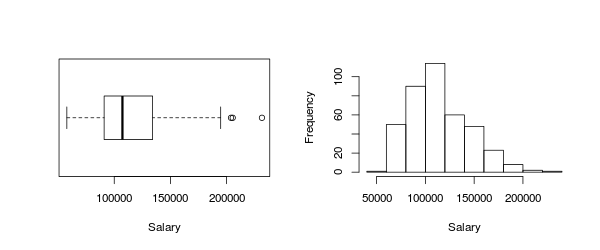
\includegraphics[width=.8\linewidth]{../../plots/salaryBoxHist.png}
  \begin{enumerate}
    \item  Is salary skewed (if so which way?) or does it have a
      symmetric distribution? 
\begin{students}
    \vspace{1cm}    
\end{students}

\begin{key}
  {\it  right skewed}
\end{key}

    \item Are any points flagged as outliers?  If so, describe them. 
\begin{students}
    \vspace{1cm}    
\end{students}

\begin{key}
  {\it Three points with salary over \$200,000 are flagged as outliers.}
\end{key}
     \item  Give approximate values for the median and the first and
       third quartiles.  Also compute the IQR.
\begin{students}
    \vspace{1cm}    
\end{students}

\begin{key}
  {\it  Q1: \$90k, Mdedian: \$110k, Q3: \$135K, IQR: \$25k}
\end{key}
    \item For these data, which is a better summary: mean and standard
      deviation?  or median and IQR? Why?
\begin{students}
    \vspace{1cm}    
\end{students}

\begin{key}
  {\it median and IQR -- due to skewness.}
\end{key}
    \end{enumerate}


  \item In Christian Rudder's book {\it Dataclysm} (2014) he shows
    plots of how men rate the attractiveness of women (data from the
    online dating site OKcupid) on a scale of 1 to 5 -- the solid line
    in this plot.  Y axis is the percentage of women who get this
    ranking. The line connects what would be the centers at the top of
    each bar of a histogram, (sometimes called a ``hollow
    Histograms'').  The dashed line was added by forcing in a
    perfectly symmetric distribution. Describe the skew of the solid
    line using the dashed line as a reference.


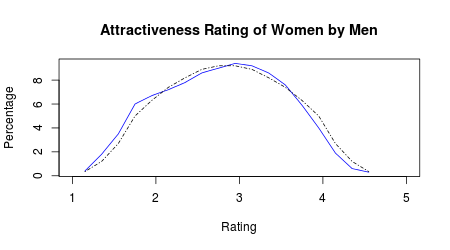
\includegraphics[width=.4\linewidth]{../../plots/menRateWomen.png}

\begin{students}
   \   \vspace{1cm}    
\end{students}

\begin{key}
  {\it The solid line is slightly skewed to the right. If womens'
    looks are symmetrically distributed, then men are being a bit hard
  on them, pushing their scores a bit lower.}
\end{key}


\item So men have some ``biases'' about female attractiveness.  What
  if we go the other way and have women rate men?  Are the men using
  OKcupid really ugly?  Describe what's going on here.

 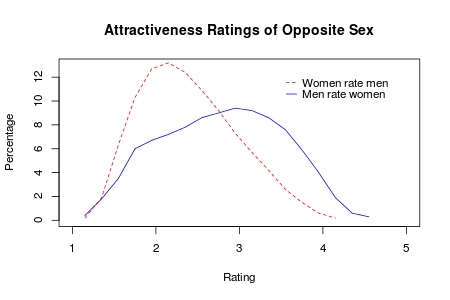
\includegraphics[width=.5\linewidth]{../../plots/RateMenAndWomen.png}
\begin{students}
\vspace{1in}
\end{students}

\begin{key}
  {\it  Women have stricter standards in what they see as attractive?
     Or are women posting pictures that are showing themselves to
     better advantage than the pictures men choose?}
\end{key}
\end{enumerate}
  



\begin{center}
  {\bf Take Home Message:}
\end{center}
\begin{itemize}
\item To learn about the world, we collect data. Two main types:
  \begin{itemize}
  \item Categorical -- summarize with proportions
  \item Quantitative -- describe center (mean or meadian) spread (SD
    or IQR) and shape of distribution (symmetric, left-skewed,
    right-skewed). 
  \end{itemize}
\item Plots:
  \begin{itemize}
  \item Categorical -- use bar charts. Pie charts waste ink and are
    harder to read.
  \item Quantitative -- Dot plots, histograms, boxplots.\\
    We describe center (mean or median), spread, and shape based on
    these plots.
  \end{itemize}
\end{itemize} \vspace{1in}



{\bf Assignment}
\begin{itemize}
\item  Quizork 1 - Descriptives\\
  A template is posted on D2L.
  Your completed Quizorks must be exported as a pdf file and uploaded
  to the D2L dropbox for Quizork2.
\item Read page 18 -- 19  for the next class.
\item View the video ``How to create a boxplot''
\end{itemize}

